\documentclass[12pt,letterpaper]{article}
\usepackage[utf8]{inputenc}
\usepackage[spanish]{babel}
\usepackage{graphicx}
\usepackage[left=2cm,right=2cm,top=2cm,bottom=2cm]{geometry}
\usepackage{graphicx} % figuras
% \usepackage{subfigure} % subfiguras
\usepackage{float} % para usar [H]
\usepackage{amsmath}
%\usepackage{txfonts}
\usepackage{stackrel} 
\usepackage{multirow}
\usepackage{enumerate} % enumerados
\usepackage{changepage}
\usepackage{amsmath}
\usepackage[all]{xy}
\renewcommand{\labelitemi}{$-$}
\renewcommand{\labelitemii}{$\cdot$}

% \author{}
% \title{Caratula}
\begin{document}

% Fancy Header and Footer
% \usepackage{fancyhdr}
% \pagestyle{fancy}
% \cfoot{}
% \rfoot{\thepage}
%

% \usepackage[hidelinks]{hyperref} % CREA HYPERVINCULOS EN INDICE

% \author{}
\title{Caratula}

\begin{titlepage}
\begin{center}
\large{UNIVERSIDAD PRIVADA DE TACNA}\\
\vspace*{-0.025in}
\begin{figure}[htb]
\begin{center}
\vspace{\baselineskip}

\includegraphics[width=4.5cm]{./Imagenes/logo}
\end{center}
\end{figure}
\vspace*{0.15in}
INGENIERIA DE SISTEMAS  \\

\vspace*{0.5in}
\begin{large}
TITULO:\\
\end{large}

\vspace*{0.1in}
\begin{Large}
\textbf{INFORME LABORATORIO 06} \\
\end{Large}

\vspace*{0.3in}
\begin{Large}
\textbf{CURSO:} \\
\end{Large}

\vspace*{0.1in}
\begin{large}
BASE DE DATOS II\\
\end{large}

\vspace*{0.3in}
\begin{Large}
\textbf{DOCENTE:} \\
\end{Large}

\vspace*{0.1in}
\begin{large}
 ING. Patrick Cuadros Quiroga\\
\end{large}

\vspace*{0.2in}
\vspace*{0.1in}
\begin{large}
Integrantes: \\
\vspace{\baselineskip}
\begin{flushleft}
Condori Gutierrez, Flor de Maria            	\hfill	(2015053227) \\
Salamanca Contreras, Fiorella Rosmery		\hfill	(2015053237) \\
Escalante Maron, Nelia		\hfill	(2014049551) \\
Coaquira Calizaya, Yerson		\hfill	(2015053225) \\
\end{flushleft}
\end{large}
\end{center}

\end{titlepage}

\tableofcontents % INDICE
\thispagestyle{empty} % INDICE SIN NUMERO
\newpage
\setcounter{page}{1} % REINICIAR CONTADOR DE PAGINAS DESPUES DEL INDICE

\section{Respuesta al ejecutar los siguientes comandos} 
\vspace{\baselineskip}
¿Qué sucede al ejecutar los siguientes comandos?
\begin{center}
	
\includegraphics[width=8cm]{./Imagenes/1} 
\end{center}

\begin{itemize}
	\item STARTUP OPEN
\end{itemize}
\begin{adjustwidth}{0.40in}{0.0in}
	Una base de datos Oracle puede estar en uno de estos cuatro estados:
	OPEN: La base de datos está completamente funcional. Para ello se abren los archivos de datos y los Redo Log y se comprueba la consistencia de los datos.\\ \\
	Este es el valor por defecto para arrancar, montar y abrir una base datos.\\ \\
	Abrir la base de datos incluyendo las siguientes tareas:	
	\begin{itemize}
		\item[$*$] Apertura de los archivos de datos en línea.
		\item[$*$] Apertura de los archivos de registro de rehacer en línea.\\
\\
	\end{itemize}		
\end{adjustwidth}

\begin{itemize}
	\item STARTUP MOUNT 
\end{itemize}
\begin{adjustwidth}{0.40in}{0.0in}
	Una base de datos Oracle puede estar en uno de estos cuatro estados:
	MOUNT: Al estado anterior se añade la lectura de los archivos de control que permiten determinar cómo se ha de preparar la instancia. Se buscan los archivos de datos y los Redo Log, comprobando su existencia en las rutas marcadas por el archivo de control.\\ \\
	En este estado podemos conectar (como administradores) y realizar tareas como:
	\begin{itemize}
		\item[$*$] Cambio del nombre de los archivos de datos.
		\item[$*$] Activar el modo ARCHIVELOG.
		\item[$*$] Recuperación de la base de datos
		\item[$*$] En definitiva, tareas sobre los archivos de la base de datos ya que aun no se han abierto sus datos.	\\
\\
	\end{itemize}
	Arrancamos la base de datos montada, normalmente se usa en modo para tareas de mantenimiento.	
\end{adjustwidth}

\begin{itemize}
	\item STARTUP NOMOUNT 
\end{itemize}
\begin{adjustwidth}{0.40in}{0.0in}
	Una base de datos Oracle puede estar en uno de estos cuatro estados: \\ \\
	NOMOUNT: La instancia de base de datos está latente en memoria, con los procesos comunes funcionando. Se abre el archivo de parámetros, se asigna en memoria el espacio para la SGA, se lanzan los procesos en segundo plano, se abren los archivos de traza y alerta.\\ \\
	Arrancamos la base de datos (instancia) pero sin montarla, se suele usar la fase de creación de una base de datos.\\ \\
	Una instancia se inicia normalmente solo en modo Nomount durante:
	\begin{itemize}
		\item[$*$] Creación de base de datos
		\item[$*$] Recreación de archivos de control.
		\item[$*$] Ciertos escenarios de copia de seguridad y recuperación.\\

	\begin{center}
		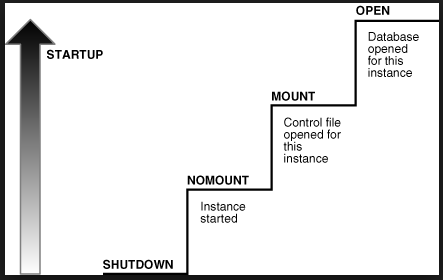
\includegraphics[width=15.3cm]{./Imagenes/startup}
	\end{center}

	\end{itemize}
\end{adjustwidth}

\begin{itemize}
	\item STARTUP FORCE  
\end{itemize}
\begin{adjustwidth}{0.40in}{0.0in}
	Arranque con un fichero de parámetros distinto al habitual o localizado en una situación diferente a donde se encuentra por defecto.\\ \\
	Si la base de datos está abierta, FORCE apaga la base de datos con una SHUTDOWN ABORT declaración antes de volver a abrirla. Si la base de datos está cerrada, entonces FORCE abre la base de datos.\\ \\
	Puede usar la opción de inicio de STARTUP FORCE si tiene dificultades para iniciar la base de datos de una manera normal. Por ejemplo, si un servidor de base de datos perdió energía y la base de datos se detuvo bruscamente, puede dejar la base de datos en un estado en el que sea necesario un inicio de STARTUP FORCE.\\ \\
	Este tipo de inicio normalmente no debería ser requerido, pero puede usarse si un inicio normal no funciona. STARTUP FORCE realiza un aborto de apagado y luego reinicia la base de datos.
\end{adjustwidth}

\begin{itemize}
	\item STARTUP RESTRICT  
\end{itemize}
\begin{adjustwidth}{0.40in}{0.0in}
	Es un modo especial de trabajo en el que la base de datos está abierta, pero solo se permite el acceso a usuarios con permiso RESTRICTED (lo poseen los administradores) para hacer tareas especiales de administración. Uso:\\
	\begin{center}
		\textbf{\large STARTUP RESTRICTED}		
	\end{center}
	\vspace{\baselineskip}
	Si la instancia ya estaba abierta es:\\
	\begin{center}
		\textbf{\large ALTER SYSTEM ENABLE RESTRICTED SESSION;}		
	\end{center} 

	Y si lo que queremos es desactivar el modo restringido para pasar a modo normal:\\
	\begin{center}
		\textbf{\large ALTER SYSTEM DISABLE RESTRICTED SESSION;}		
	\end{center}
	\vspace{\baselineskip}
	Arrancamos la base de datos en modo restringido, solo usuario que tengan privilegios de CREATE SESSION y RESTRICTED SESSION podrán conectarse.\\ \\
	La opción STARTUP RESTRICT inicia la base de datos y la coloca en modo ABIERTO, pero da acceso solo a los usuarios que tienen el privilegio RESTRICTED SESSION. Es posible que desee abrir una base de datos utilizando la opción RESTRINGIDA cuando desee realizar el mantenimiento de la base de datos mientras esté abierta, pero asegúrese de que los usuarios no puedan conectarse y realizar trabajos en la base de datos.\\ \\
	Es posible que también desee abrir la base de datos utilizando la opción RESTRINGIDA para realizar exportaciones o importaciones de la base de datos y garantizar que ningún usuario acceda al sistema durante estas actividades. Una vez que haya terminado con su trabajo, puede deshabilitar la sesión restringida, ALTERAR LA SESIÓN RESTRINGIDA DEL SISTEMA, para que todos puedan conectarse a la base de datos.\\
\\
	
\end{adjustwidth}

\begin{itemize}
	\item STARTUP RECOVER  
\end{itemize}
\begin{adjustwidth}{0.40in}{0.0in}
	Especifica que la recuperación de medios se debe realizar, si es necesario, antes de iniciar la instancia. STARTUP RECOVER tiene el mismo efecto que emitir el comando RECOVER DATABASE e iniciar una instancia. Solo la recuperación completa es posible con la opción RECUPERACIÓN.\\ \\
	La recuperación continúa, si es necesario, como si AUTORECOVERY estuviera en ON, independientemente de si AUTORECOVERY está habilitado o no. Si no se encuentra un archivo de registro de rehacer en la ubicación esperada, la recuperación continúa como si AUTORECOVERY estuviera deshabilitado, al indicarle la ubicación sugerida y el nombre de los archivos de registro posteriores que deben aplicarse.\\
\\
\end{adjustwidth}

\begin{itemize}
	\item SHUTDOWN NORMAL   
\end{itemize}
\begin{adjustwidth}{0.40in}{0.0in}
	Una instancia cuando es arrancada, hasta estar disponible atraviesa todos los estados anteriores.\\ 
	El comando de apagado de la instancia es SHUTDOWN, su sintaxis:\\ \\
	NORMAL: Modo en el que no se admiten más conexiones a la base de datos, pero las actuales se mantienen. Cuando se cierre la última sesión, la base de datos pasará a estar cerrada (SHUTDOWN), pero, hasta entonces, seguirá abierta. Al cerrar se fuerza un checkpoint y se graban todos los datos del búfer, además de cerrarse los archivos.\\ \\
	Caracteristicas:
	\begin{itemize}
		\item[$*$] Espera a que los usuarios conectados actualmente finalicen TODAS las operaciones.
		\item[$*$] Evita nuevas conexiones. Los usuarios que intentan conectarse reciben el mensaje "Shutdown in progress".
		\item[$*$] Cierra y desmonta la B.D. Cierra la SGA para los procesos background.
		\item[$*$] No necesita recuperacion al arrancar la base de datos.\\ \\
	\begin{center}
		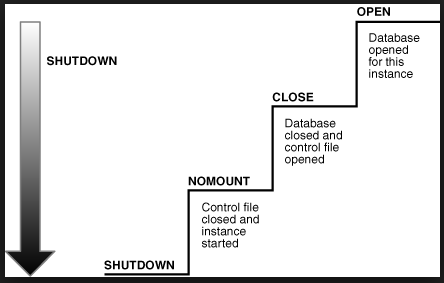
\includegraphics[width=15.3cm]{./Imagenes/shutdown}
	\end{center}
	\end{itemize}	
\end{adjustwidth}

\vspace{\baselineskip}
\vspace{\baselineskip}

\section{Privilegios de sistema (DDL) utilizados del script proporcionado lab\_02\_01.sql}
\vspace{\baselineskip}
En Oracle los usuarios necesitan permisos para poder acceder a la base de datos y a los objetos de la misma. Los privilegios pueden ser de dos tipos: a) del sistema y b) sobre objetos.\\ \\
Para conceder un privilegio de sistema: "create session", que es necesario para poder conectarse a la base de datos, es decir, para iniciar una sesión.\\ \\
Pero teniendo únicamente este permiso, no podemos hacer mucho, solamente iniciar una sesión, pero no podemos crear tablas, ni ningún otro objeto; por ello son importantes los permisos de creación de objetos.
	\begin{center}
		
\includegraphics[width=10cm]{./Imagenes/2} 
	\end{center}
	Los privilegios de sistema son permisos para realizar ciertas operaciones en la base de datos.\\ \\
	En Oracle existen dos tipos de privilegios de usuario:
	\begin{itemize}
		\item[$*$] System: Que permite al usuario hacer ciertas tareas sobre la BD, como por ejemplo crear un Tablespace. Estos permisos son otorgados por el administrador o por alguien que haya recibido el permiso para administrar ese tipo de privilegio. Existen como 100 tipos distintos de privilegios de este tipo.
		\item[$*$] Object: Este tipo de permiso le permite al usuario realizar ciertas acciones en objetos de la BD, como una Tabla, Vista, un Procedure o Función, etc. Si a un usuario no se le dan estos permisos sólo puede acceder a sus propios objetos (véase USER\_OBJECTS). Este tipo de permisos los da elowner o dueño del objeto, el administrador o alguien que haya recibido este permiso explícitamente (con Grant Option).\\
\\
	\end{itemize}	
Los siguientes son algunos de los privilegios de sistema existentes:
	\begin{itemize}
		\item[$*$] create session: para conectarse a la base de datos
		\item[$*$] create table: crear tablas
		\item[$*$] create sequence: crear secuencias;
		\item[$*$] create view: crear vistas;
		\item[$*$] create trigger: crear disparadores en su propio esquema;
		\item[$*$] create procedure: crear procedimientos y funciones;
		\item[$*$] execute any procedure: ejecutar cualquier procedimiento en cualquier esquema;
		\item[$*$] create user: crear usuarios y especificar claves;
		\item[$*$] create role: crear roles;
		\item[$*$] drop user: eliminar usuarios.\\
\\
	\end{itemize}
Cada tipo de objeto tiene su propio conjunto de permisos:
	\begin{itemize}
		\item[$*$] Tables: select, insert, update, delete, alter, debug, flashback, on commit refresh, query rewrite, references, all.
		\item[$*$] Views: select, insert, update, delete, under, references, flashback, debug.
		\item[$*$] Sequence: alter, select.
		\item[$*$] Packeges, Procedures, Functions (Java classes, sources...): execute, debug.
		\item[$*$] Materialized Views: delete, flashback, insert, select, update.
		\item[$*$] Directories: read, write
		\item[$*$] Libraries:execute
		\item[$*$] User defined types: execute, debug, under
		\item[$*$] Operators: execute
		\item[$*$] Indextypes: execute\\
\\
	\end{itemize}
Concede permisos para objetos de sistema, como procedimientos almacenados del sistema, procedimientos almacenados extendidos, funciones y vistas.
\begin{center}
	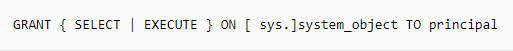
\includegraphics[width=17.5cm]{./Imagenes/3} 
\end{center}

Argumentos \\ \\
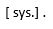
\includegraphics[width=1.5cm]{./Imagenes/sysc} \\ 
Solo se requiere el calificador sys para hacer referencia a vistas de catálogo y vistas de administración dinámica.\\ \\
system\_object\\
Especifica el objeto en el que se va a conceder el permiso.\\
Especifica la entidad de seguridad para la que se concede el permiso.\\
Se asignan privilegios de sistema a un usuario mediante la instrucción "grant":\\ \\
Sintaxis básica:\\ \\
grant PERMISODESISTEMA\\
to USUARIO;\\ \\
Oracle permite conceder múltiples privilegios a múltiples usuarios en una misma sentencia, debemos separarlos por comas.\\ \\
En el siguiente ejemplo se concede el permiso para crear sesión a los usuarios "juan" y "ana": \\
grant create sesion to juan, ana;\\ \\
En el siguiente ejemplo se conceden los permisos para crear tablas y vistas al usuario "ana":\\
grant create table, \\
create view
to ana;\\ \\
En el siguiente ejemplo se conceden 2 permisos a 2 usuarios en una sola sentencia:\\
grant create trigger,\\
create procedure to juan, ana;\\ \\
Consultando el diccionario "dba\_sys\_privs" encontramos los privilegios concedidos a los distintos usuarios; y consultando "user\_sys\_privs" obtendremos la misma información pero únicamente del usuario actual.


\section{Tipos de TableSpace que existen en Oracle.} 
\vspace{\baselineskip}
Un tablespace es una unidad lógica de almacenamiento dentro de una base de datos oracle.\\
Es un puente entre el sistema de ficheros del sistema operativo y la base de datos.\\ \\
Cada tablespace se compone de, al menos, un datafile y un datafile solo puede pertenecer a un tablespace.\\
Cada tabla o indice de oracle pertenece a un tablespace, es decir cuando se crea una tabla o indice se crea en un tablespace determinado.\\ \\
Los tablespace son estructuras donde se almacenan los objetos del esquema de la base de datos, tales como tablas, índices, etc. con la particularidad de poderse repartir en varios ficheros. Por tanto, las bases de datos tienes varios tablespaces y estos a su vez varios datafiles. Un datafile sólo pertenece a un tablespace y un tablespace sólo pertenece a una Base de Datos.
\\
\\
\\
\begin{center}
	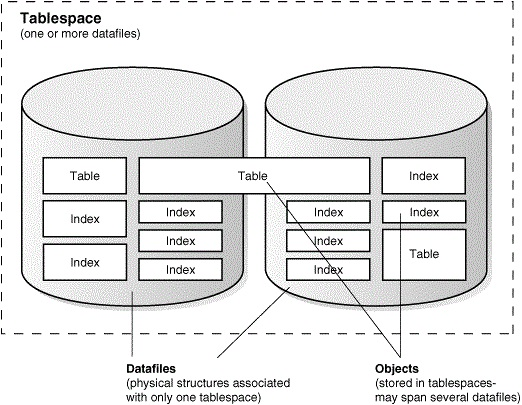
\includegraphics[width=14cm]{./Imagenes/4} 
\end{center}

\newpage

TIPOS DE TABLESPACE
\\
\begin{itemize}
	\item TABLESPACE SYSTEM:
\end{itemize}
\begin{adjustwidth}{0.40in}{0.0in}
	El espacio de tabla principal en cualquier base de datos es el tablespace SYSTEM, que contiene información básica sobre el funcionamiento del servidor de la base de datos, como el diccionario de datos y el segmento de reversión del sistema. El tablespace SYSTEM es el primer espacio de tabla creado en la creación de la base de datos. Se gestiona como cualquier otro espacio de tabla, pero requiere un mayor nivel de privilegios y está restringido de alguna manera. Por ejemplo, no puede cambiar el nombre o eliminar el tablespace SYSTEM o desconectarlo.	\\ \\
	Características:
	\begin{itemize}
		\item[$*$] Se crea automáticamente al hacer la instalación de Oracle o al crear una Base de Datos.
		\item[$*$] Contiene el diccionario de datos.\\
	\end{itemize}		
\end{adjustwidth}

\begin{itemize}
	\item TABLESPACE TEMPORALES:
\end{itemize}
\begin{adjustwidth}{0.40in}{0.0in}
	Un tablespaces temporal contiene datos transitorios que persisten solo durante la sesión. Los tablespace temporales pueden mejorar la concurrencia de múltiples operaciones de clasificación que no caben en la memoria y pueden mejorar la eficiencia de las operaciones de gestión de espacio durante las clasificaciones.\\ \\
	Los tablespace temporales se utilizan para almacenar lo siguiente:
	\begin{itemize}
		\item[$*$] Resultados de clasificación intermedios.
		\item[$*$] Tablas temporales e índices temporales.
		\item[$*$] LOB's temporales.
		\item[$*$] Árboles B temporales.\\
	\end{itemize}
	Dentro de un espacio de tabla temporal, todas las operaciones de clasificación para una instancia particular comparten un único segmento de clasificación, y existen segmentos de clasificación para cada instancia que realiza operaciones de clasificación que requieren espacio temporal. La primera instrucción después de la puesta en marcha crea un segmento de clasificación que utiliza el espacio de tabla temporal para la clasificación, y se libera solo en el cierre.\\ \\
	Características:
	\begin{itemize}
		\item[$*$] Es aquél en el que solamente puede haber objetos temporales. No se pueden crear objetos permanentes como pueden ser los índices, las tablas o los segmentos de rollback.
		\item[$*$] Optimización operaciones de ordenación.\\
	\end{itemize}		
\end{adjustwidth}

\newpage

\begin{itemize}
	\item TIPO BIGFILE (10g):
\end{itemize}
\begin{adjustwidth}{0.40in}{0.0in}
	Un tablespace bigfile es un tablespace con un archivo de datos único, pero muy grande (hasta bloques 4G). Los tablespace tradicionales de archivos pequeños, por el contrario, pueden contener varios archivos de datos, pero los archivos no pueden ser tan grandes. Los beneficios de los tablespace de bigfile son los siguientes:
	\begin{itemize}
		\item[$*$] Un espacio de tabla de bigfile con bloques de 8K puede contener un archivo de datos de 32 terabytes. 
		\item[$*$] Los tablespace de bigfile pueden reducir la cantidad de archivos de datos necesarios para una base de datos. 
		\item[$*$] Los tablespace de bigfile simplifican la administración de la base de datos al proporcionar transparencia de archivos de datos. \\
	\end{itemize}
	Los tablespace de Bigfile solo se admiten para tablespace administrados localmente con administración de espacio de segmento automática, con tres excepciones: tablespace deshacer gestionados localmente, tablespace temporales y el tablespace SYSTEM.		
\end{adjustwidth}

\begin{itemize}
	\item TIPO SMALL-FILE (10g):
\end{itemize}
\begin{adjustwidth}{0.40in}{0.0in}
	Utilice esta cláusula para determinar si el espacio de tabla es un espacio de tabla de bigfile o smallfile. Esta cláusula anula cualquier configuración de tipo de espacio de tabla predeterminada para la base de datos.\\ \\		
	Un tablespace SmallFile es un espacio de tabla de Oracle tradicional, que puede contener 1022 archivos de datos o archivos temporales, cada uno de los cuales puede contener hasta aproximadamente 4 millones (2~22)de bloques.\\ \\	
	Un tablespace SmallFile muy diferente de un espacio de tabla de archivo grande.El tablespace SmallFile es el espacio de tabla "tradicional" de Oracle, y la distinción solo se hizo en 10 g con la introducción del tablespace de bigfile.\\ \\	
	El valor predeterminado para los tipos de espacios de tablas es un espacio de tablas de pequeño tamaño, pero el valor predeterminado se puede cambiar al crear la base de datos:\\\\
\\
	\begin{center}
		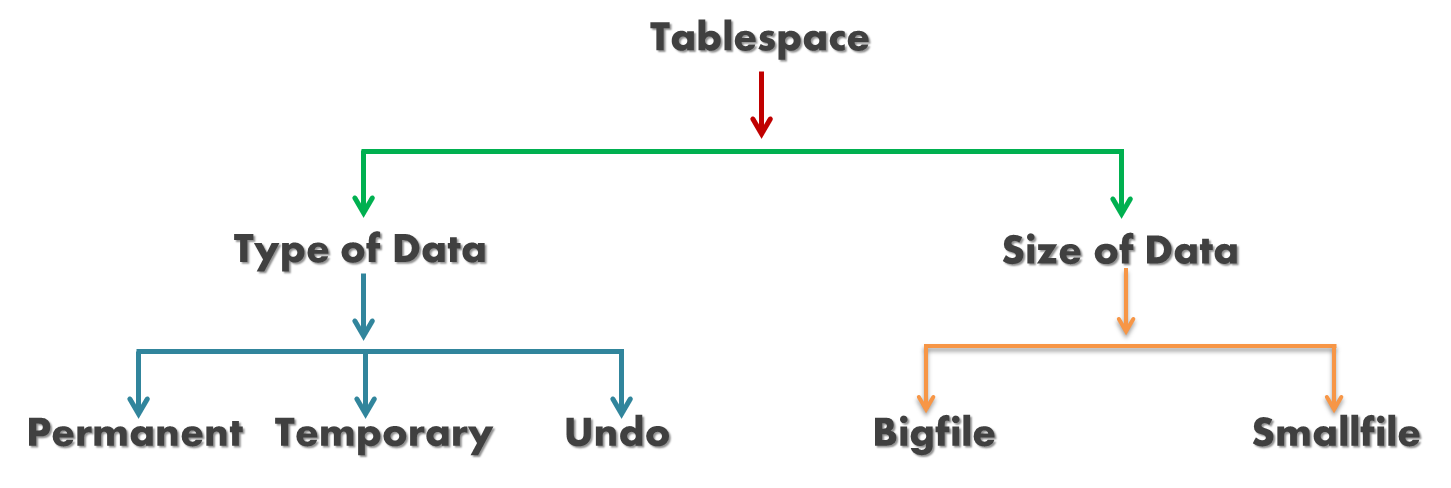
\includegraphics[width=15.3cm]{./Imagenes/5}
	\end{center}
\end{adjustwidth}

\vspace{\baselineskip}

\begin{itemize}
	\item TABLESPACE READ-ONLY:
\end{itemize}
\begin{adjustwidth}{0.40in}{0.0in}
	La creación de un tablespace de solo lectura evita las operaciones de escritura en los archivos de datos en el tablespace. El propósito principal de los espacios de tabla de solo lectura es eliminar la necesidad de realizar copias de seguridad y recuperación de grandes porciones estáticas de una base de datos.\\ \\
	Los espacios de tabla de solo lectura también proporcionan una forma de proteger los datos históricos para que los usuarios no puedan modificarlos. La creación de un tablespace de solo lectura evita actualizaciones en todas las tablas del tablespace, independientemente del nivel de privilegio de actualización del usuario.\\ \\	
	Se pueden consultar los datos de los objetos, no se puede ni borrar ni insertar nada en ellos. La principal ventaja de un tablespace read-only es que no hace falta hacer backup del mismo.\\
\end{adjustwidth}

\vspace{\baselineskip}

\end{document}
